\section*{Background}
\subsection*{The Problem}
The interest in studying rodent whiskers has recently seen a significant increase, particularly in the field of neurophysiology. As a result, there is a need for automatic tracking of whisker movements. Currently available commercial solutions either are extremely expensive, restrict the experiment setup\footnote{A method known as \emph{optoelectronic monitoring} takes this to the extreme by having the rat locked in place by cranium-mounted screws \cite{Optoelectronic}. See figure \ref{fig:optoelectronic}.}, or fail in \emph{clutter}ed environments or when whiskers occlude each other\footnote{A system developed by Volgts, Sakmann and Celikel manages to track $\leq 8$ whiskers on each face side, but has difficulties tracking more whiskers than that \cite{UnsupervisedTracking}.}. A cheap, reliable solution to the tracking problem is needed.

\begin{figure}[h]
  \centering
  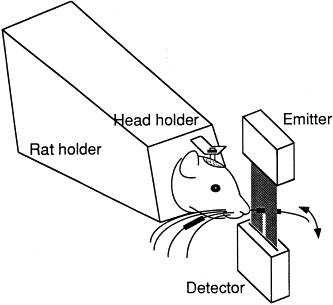
\includegraphics[width=0.3\textwidth]{optoelectronic.png}
  \caption{A very restrained experiment setup.}
  \label{fig:optoelectronic}
\end{figure}

\begin{figure}
  \centering
  \begin{tabular}{rl}
    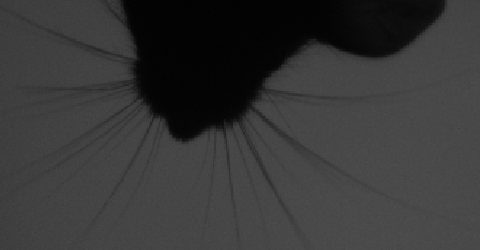
\includegraphics[width=0.5\textwidth]{rat-vanilla.png}
    & 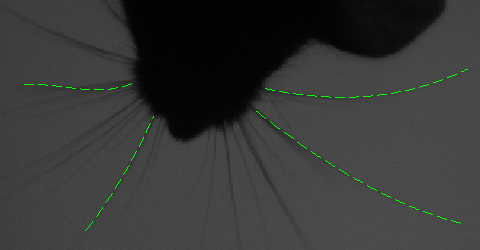
\includegraphics[width=0.5\textwidth]{rat-splines.png}
    \label{fig:rat}
  \end{tabular}

  \caption{Left: Example image of a rat and its whiskers. Right: Least squares fitted third degree polynomials.}
  \label{fig:whiskers}
\end{figure}

\subsection*{A Probabilistic Approach}
We propose solving the problem by a probabilistic approach. We use a technique known as the \emph{Particle Filter} to propagate a whisker model between frames of high speed video. In each frame, the next state of the model is predicted by searching a pre-trained database, and filtering the results through the Particle Filter. The main difference between this and existing solutions is that it maintains a model of the whiskers. This makes it easier to keep track of them even in the presence of clutter.
